\begin{flushright}
    \section*{\Large{Ujian Akhir Semester}}
    \addcontentsline{toc}{section}{Ujian Akhir Semester (UAS)}
    \subsection*{Tahun 2020}
    \addcontentsline{toc}{subsection}{UAS - 2020}
\end{flushright}


\vspace{0.5cm}\hrule height 2pt\vspace{0.5cm}


\begin{center}
\textbf{\large{MATERI}}
\begin{enumerate}[leftmargin=*, label={\arabic*}.]
\item Teknik-teknik Integrasi
\item Sketsa grafik fungsi dan kurva.
\item Aplikasi integral dalam mencari volume benda putar.
\item Fungsi Logaritma dan Eksponensial
\item Fungsi Invers
\end{enumerate}
\end{center}


\vspace{0.2cm}\hrule height 1pt\vspace{0.5cm}


\begin{center}
\textbf{\large{SOAL}}
\end{center}
\begin{enumerate}[leftmargin=*, label={\arabic*}.]
\item Tentukanlah
    \begin{enumerate}[label={\alph*}.]
    \item $\ds\int \frac{x\sin\sqrt{x^{2}+4}}{\sqrt{x^{2}+4}}\, dx$
    \item $\ds\int_{-\pi/2}^{\pi/2} \cos\theta\cos\brk*{\pi\sin\theta}\,d\theta$
    \end{enumerate}
\item Daerah $R$ yang dibatasi oleh $y=3x^{2}-2$, $y=x^{2}$, dan $x\geq 0$, diputar 
mengelilingi sumbu-$y$.
    \begin{enumerate}[label={\alph*}.]
    \item Sketsalah daerah $R$.
    \item Metode apa sajakah yang dapat digunakan untuk menghitung volume benda putar 
    yang terbentuk?
    \item Hitunglah volume benda putar tersebut dengan menggunakan salah satu metode yang 
    Anda sebutkan pada bagian b!
    \end{enumerate}
\item Diberikan fungsi bernilai real $f$ dan $g$ sebagai berikut:
\[
f(x)=3+\sqrt{\frac{1}{x-1}}\,\text{ dengan }x > 1\,\text{dan }g(x)=
\int_{x}^{0}\sqrt{\frac{1}{4}+\sin^{2}t}\,dt.
\]
    \begin{enumerate}[label={\alph*}.]
    \item Tentukanlah $f^{-1}(x)$, kemudian carilah $(f^{-1})'(x)$.
    \item Jika $p=g(a)$, $0\leq a \leq \frac{\pi}{2}$, tentukanlah nilai $a$ 
    yang memenuhi persamaan:
    \[
    (f^{-1})'(4)=(g^{-1})'(p).
    \]
    \end{enumerate}
\item Hitunglah
    \begin{enumerate}[label={\alph*}.]
    \item Jika $f(x)=\sin^{2}x+2^{\sin x}$, maka $2e^{f'(\pi)}=\dots$.
    \item $\int_{0}^{1} 10^{3x}+10^{-3x}\,dx$.
    \end{enumerate}
\item Tentukanlah
    \begin{enumerate}[label={\alph*}.]
    \item $\int \arctan(5x)\,dx$.
    \item $\ds \int \frac{1}{\brk*{x^{2}+4}^{3/2}}\,dx$ 
    $\ds\brk*{\text{petunjuk: } \sin(\arctan x) = \frac{x}{\sqrt{1+x^{2}}}}$.
    \end{enumerate}
\end{enumerate}


\vspace{0.2cm}\hrule height 1pt\vspace{0.5cm}


\begin{center}
\textbf{\large{PEMBAHASAN}}
\end{center}
\begin{enumerate}[leftmargin=*, label={\arabic*}.]
\item Gunakan metode subtitusi untuk menyelesaikan integral-integral berikut
    \begin{enumerate}[label={\alph*}.]
    \item $\ds\int \frac{x\sin\sqrt{x^{2}+4}}{\sqrt{x^{2}+4}}\, dx$
    
    Subtitusi
    \[
        u = \sqrt{x^{2}+4},\quad\frac{du}{dx} = \frac{1}{2}\frac{1}{\sqrt{x^{2}+4}}(2x) 
        \iff du = \frac{x}{\sqrt{x^{2}+4}}\,dx
    \]
    Sehingga 
    \begin{align*}
        &\int \frac{x\sin\sqrt{x^{2}+4}}{\sqrt{x^{2}+4}}\, dx \\
        =\,& \int \sin\sqrt{x^{2}+4}\frac{x}{\sqrt{x^{2}+4}}\, dx\\
        =\,& \int \sin u\, du\\
        =\,&-\cos u + C\\
        =\,&-\cos\sqrt{x^{2}+4} + C &\text{subtitusi balik }u = \sqrt{x^{2}+4}
    \end{align*}

    $\therefore$ 
    $\ds\int \frac{x\sin\sqrt{x^{2}+4}}{\sqrt{x^{2}+4}}\, dx = -\cos\sqrt{x^{2}+4} + C$


\begin{center}\line(1,0){150}\end{center}


    \item $\ds\int_{-\pi/2}^{\pi/2} \cos\theta\cos\brk*{\pi\sin\theta}\,d\theta$
    
    Subtitusi
    \begin{align*}
        &u = \sin\theta,&\frac{du}{d\theta} = \cos\theta \iff du = \cos\theta\,d\theta\\
        &x=-\frac{\pi}{2} \iff u = \sin\brk*{-\frac{\pi}{2}} = -1,
        &x=\frac{\pi}{2} \iff u = \sin \brk*{\frac{\pi}{2}} = 1
    \end{align*}
    Sehingga 
    \begin{align*}
        &\int_{-\pi/2}^{\pi/2} \cos\theta\cos\brk*{\pi\sin\theta}\,d\theta\\
        =\,& \int_{-\pi/2}^{\pi/2} \cos\brk*{\pi\sin\theta}\cos\theta\,d\theta\\
        =\,& \int_{-1}^{1} \cos(\pi u)\, du\\
        =\,& \eval{\frac{\sin(\pi u)}{\pi}}{-1}{1}\\
        =\,& \frac{\sin\pi}{\pi}-\frac{\sin(-\pi)}{\pi} = 0
    \end{align*}

    $\therefore$ $\ds\int_{-\pi/2}^{\pi/2} \cos\theta\cos\brk*{\pi\sin\theta}\,d\theta = 0$
    
    \end{enumerate}

\begin{center}\line(1,0){300}\end{center}


\item Diberikan daerah $R$ yang dibatasi oleh $y=3x^{2}-2$, $y=x^{2}$, dan $x\geq 0$, diputar 
mengelilingi sumbu-$y$.
    \begin{enumerate}[label={\alph*}.]
    \item Akan disketsa daerah $R$.
    
    Gunakan tiga titik dari masing-masing persamaan untuk mensketsa kurva.
    \begin{center}
        \begin{tabular}{|c|c|c|c|}\hline
            $x$ & $-1$ & $0$ & $1$ \\ \hline
            $y=x^2$ & $1$ & $0$ & $1$ \\ \hline
        \end{tabular}\quad
        \begin{tabular}{|c|c|c|c|}\hline
            $x$ & $-1$ & $0$ & $1$ \\ \hline
            $y=3x^{2}-2$ & $1$ & $-2$ & $1$ \\ \hline
        \end{tabular}
    \end{center}
    Diperoleh daerah yang dibatasi seperti berikut:
    
    \begin{center}
\begin{tikzpicture}[>=stealth]
\begin{axis}[
    xmin=-2,xmax=2,
    ymin=-2.2,ymax=2,
    axis x line=middle,
    axis y line=middle,
    axis line style=<->,
    xlabel={$x$},
    ylabel={$y$},
    ]
    
    \addplot [name path=f, no marks,blue, domain=-2:2,samples=50]({x},{x^2});
    \node [blue] at (-0.5,0.7){\scalebox{0.7}{$y=x^{2}$}};
    \addplot [name path=g, no marks,red, domain=-2:2,samples=50]({x},{3*x^2-2});
    \node [red] at (1.4,0.5){\scalebox{0.7}{$y=3x^{2}-2$}};
    
    \point{blue}{(0,0)};
    \point{red}{(0,-2)};
    \point{purple}{(-1,1)};
    \point{purple}{(1,1)};
    
    \addplot [thick, color=cyan, fill=cyan, fill opacity=0.5]
        fill between[of=f and g, soft clip={domain=0:1},]; 
\end{axis}
\end{tikzpicture}
\end{center}

    $\therefore$ Telah disketsa daerah $R$.


\begin{center}\line(1,0){150}\end{center}


    \item Metode apa saja yang dapat digunakan untuk menghitung volume benda putar?
    \item 
    Apabila partisi dilakukan sejajar dengan sumbu-$y$ metode kulit tabung dapat digunakan. 
    Bila partisi dilakukan tegak lurus dengan sumbu-$y$ metode cakram digabung cincin dapat 
    digunakan.

    $\therefore$ Untuk menghitung volume benda putar yang terbentuk dapat digunakan metode 
    kulit tabung atau metode cakram + cincin.


\begin{center}\line(1,0){150}\end{center}


    \item Sebelum menghitung volume akan ditentukan batas atas, bawah, kanan, kiri daerah $R$.\\
    Batas kirinya adalah $x=0$ karena dibatasi oleh $x\geq 0$.\\
    Batas bawah adalah perpotongan 
    $y=3x^{2}-2$ dengan sumbu-$y$ ($x=0$) yaitu pada titik $(0,-2)$.\\
    Batas atas sekaligus batas kanannya adalah perpotongan $y=x^{2}$ dan $y=3x^{2}-2$.
    \begin{align*}
        y=x^{2},y=3x^{2}-2 &\Longrightarrow x^{2}=3x^{2}-2\\
        &\iff 2x^{2}-2 = 0\\
        &\iff x^{2}-1=0\\
        &\iff (x-1)(x+1)=0
    \end{align*}
    Sehingga batas atas dan kanan daerah $R$ adalah titik saat $x=1$ yaitu $(1,1)$
    
    Pertama akan dihitung volume benda putar dengan metode \textbf{kulit tabung}. 
    Partisi sejajar sumbu-$y$.\\
    Tinggi tabung dibatas di atas oleh $y=x^{2}$ dan dibatas di bawah $y=3x^{2}-2$, 
    sehingga tinggi tabung adalah $x^{2}-(3x^{2}-2)=2-2x^{2}$.\\
    Jari-jari tabung adalah jarak sumbu-$y$ ke masing-masing partisi, sehingga 
    jari-jari tabung adalah $x$ untuk $0 \leq x \leq 1$ (batas kiri -- batas kanan).\\
    Gunakan integral untuk menghitung volume

    \begin{align*}
        V &= \int \text{Luas Kulit Tabung}\\
        &=\int_{0}^{1} 2\pi(\text{jari-jari})(\text{tinggi})\,dx\\
        &=2\pi\int_{0}^{1} (x)(2-2x^{2})\,dx\\
        &=4\pi\int_{0}^{1} x-x^{3}\,dx\\
        &=4\pi\eval{\frac{1}{2}x^{2}-\frac{1}{4}x^{4}}{0}{1}\\
        &=4\pi\brk*{\brk*{\frac{1}{2}(1)^{2}-\frac{1}{4}(1)^{4}}-(0)}\\
        &=4\pi\frac{1}{4} = \pi
    \end{align*}
    
    Kedua akan dihitung volume benda putar dengan metode \textbf{cakram + cincin}.\\ 
    Partisi tegak lurus sumbu-$y$.\\
    Metode Cakram digunakan pada daerah $R$ dimana $-2 \leq y \leq 0$.\\
    Jari-jari cakram adalah jarak dari $y=3x^{2}-2$ ke sumbu-$y$.
    Jarak dibutuhkan dalam $x$ sehingga
    \[
    y=3x^{2}-2 \iff y+2 = 3x^{2} \iff x^{2}=\frac{y+2}{3}
    \]
    Gunakan integral untuk menghitung volume

    \begin{align*}
        V_I &= \int \text{Luas Cakram}\\
        &=\int_{-2}^{0} \pi(\text{jari-jari})^2\,dy\\
        &=\pi\int_{-2}^{0} \frac{y+2}{3}\,dy\\
        &=\frac{\pi}{3}\int_{-2}^{0} y+2\,dy\\
        &=\frac{\pi}{3}\eval{\frac{1}{2}y^{2}+2y}{0}{-2}\\
        &=\frac{\pi}{3}\brk*{(0)-\brk*{\frac{1}{2}(-2)^{2}+2(-2)}}\\
        &=\frac{2\pi}{3}
    \end{align*}
    Metode Cincin digunakan pada daerah $R$ dimana $0 \leq y \leq 1$.\\
    Jari-jari luar cincin adalah jarak dari $y=3x^{2}-2$ ke sumbu-$y$.\\
    Jari-jari dalam cincin adalah jarak dari $y=x^{2}$ ke sumbu-$y$.\\
    Jarak dibutuhkan dalam $x$ sehingga
    \[
        y=3x^{2}-2 \iff x^{2}=\frac{y+2}{3}\quad \text{dan} \quad y=x^{2} \iff x^{2}=y
    \]
    Gunakan integral untuk menghitung volume

    \begin{align*}
        V_{II} &= \int \text{Luas Bagian Luar} - \text{Luas Bagian Dalam}\\
        &=\int_{0}^{1} \pi(\text{jari-jari luar})^2 - \pi (\text{jari-jari dalam})^{2}\,dy\\
        &=\pi \int_{0}^{1} \brk*{\frac{y+2}{3}} -(y)\,dy\\
        &=\frac{\pi}{3}\int_{0}^{1} 2-2y\,dy\\
        &=\frac{\pi}{3}\eval{2y-y^{2}}{0}{1}\\
        &=\frac{\pi}{3}\brk*{\brk*{2(1)-(1)^{2}}-(0)}\\
        &=\frac{\pi}{3}
    \end{align*}
    Sehingga 
    \[
        V = V_{I}+V_{II} = \frac{2\pi}{3}+\frac{\pi}{3} = \pi
    \]
    Berikut ilustrasi hasil benda padat

    \begin{center}
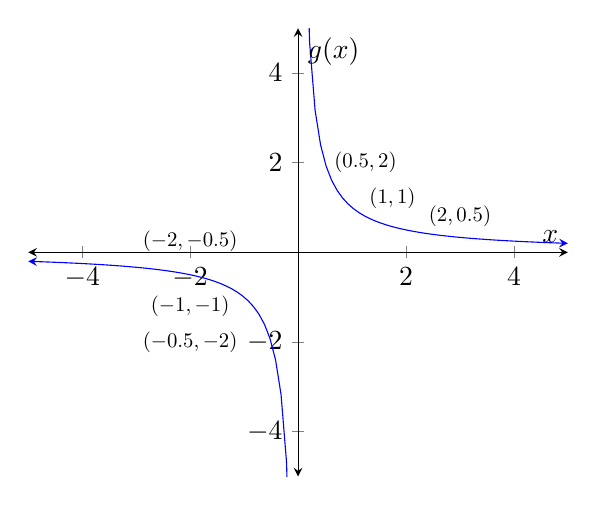
\begin{tikzpicture}[>=stealth]
\begin{axis}[
    xmin=-5,xmax=5,
    ymin=-5,ymax=5,
    axis x line=middle,
    axis y line=middle,
    axis line style=<->,
    xlabel={$x$},
    ylabel={$g(x)$},
    ]
    \addplot[no marks,blue, <-] 
        expression[domain=-5:-0.01,samples=50]{1/x} 
        node[pos=0,anchor=south west]{};
    \addplot[no marks,blue, ->] 
        expression[domain=0.01:5,samples=50]{1/x} 
        node[pos=0,anchor=south west]{};

    \point{black}{(0.5,2)};
    \point{black}{(1,1)};
    \point{black}{(2,0.5)};
    \node at (1.25,2) {\scalebox{0.75}{$(0.5,2)$}};
    \node at (1.75,1.2) {\scalebox{0.75}{$(1,1)$}};
    \node at (3,0.8) {\scalebox{0.75}{$(2,0.5)$}};

    \point{black}{(-0.5,-2)};
    \point{black}{(-1,-1)};
    \point{black}{(-2,-0.5)};
    \node at (-2,-2) {\scalebox{0.75}{$(-0.5,-2)$}};
    \node at (-2,-1.2) {\scalebox{0.75}{$(-1,-1)$}};
    \node at (-2,0.25) {\scalebox{0.75}{$(-2,-0.5)$}};
\end{axis}
\end{tikzpicture}
\end{center}
    
    $\therefore$ Diperoleh volume benda putar tersebut adalah $\pi$ baik menggunakan kulit tabung 
    maupun cincin dan cakram.

    \end{enumerate}

\begin{center}\line(1,0){300}\end{center}


\item Diberikan fungsi bernilai real $f$ dan $g$ sebagai berikut:
\[
f(x)=3+\sqrt{\frac{1}{x-1}}\,\text{ dengan }x > 1\,\text{dan }g(x)=
\int_{x}^{0}\sqrt{\frac{1}{4}+\sin^{2}t}\,dt.
\]
    \begin{enumerate}[label={\alph*}.]
    \item Pertama akan dicari $f^{-1}(x)$.
    Misalkan $y=f(x)$, maka
    \begin{align*}
        &y = 3+\sqrt{\frac{1}{x-1}}\\
        \iff &y-3 = \sqrt{\frac{1}{x-1}}\\
        \iff &(y-3)^{2} = \brk*{\sqrt{\frac{1}{x-1}}}^2\\
        \iff &(y-3)^{2} = \abs*{\frac{1}{x-1}}\\
        \iff &(y-3)^{2} = \frac{1}{x-1}
        &\text{karena }x>1\\
        \iff &x-1=\frac{1}{(y-3)^{2}}\\
        \iff &x=\frac{1}{(y-3)^{2}}+1
    \end{align*}
    Sehingga
    \[
    f^{-1}(y) = x = \frac{1}{(y-3)^{2}}+1
    \]
    Kedua akan dicari $(f^{-1})'(x)$.
    \[
        (f^{-1})'(x) = \drv{x}{f^{-1}(x)}
        = \drv{x}{\frac{1}{(x-3)^{2}}+1}=\frac{(-2)}{(x-3)^{3}}
    \]

    $\therefore$ Diperoleh $\ds f^{-1}(x) = \frac{1}{(x-3)^{2}}+1$ dan 
    $\ds (f^{-1})'(x) =-\frac{2}{(x-3)^{3}}$.


\begin{center}\line(1,0){150}\end{center}


    \item Diberikan $p=g(a)$, $0\leq a \leq \frac{\pi}{2}$, akan dicari nilai $a$ 
    yang memenuhi persamaan:
    \[
    (f^{-1})'(4)=(g^{-1})'(p).
    \]
    Pertama
    \[
        (f^{-1})'(4)=-\frac{2}{(4-3)^{3}} = -2
    \]
    Sebelum lanjut, carilah $g'(x)$ dengan menggunakan Teorema Dasar Kalkulus.
    \begin{align*}
        g'(x) &= \drv{x}{\int_{x}^{0}\sqrt{\frac{1}{4}+\sin^{2}t}\,dt}\\
        &= \drv{x}{-\int_{0}^{x}\sqrt{\frac{1}{4}+\sin^{2}t}\,dt}\\
        &= -\sqrt{\frac{1}{4}+\sin^{2}x}\\
    \end{align*}
    Kedua, dengan Teorema Turunan Invers dan Teorema Dasar Kalkulus
    \[
        (g^{-1})'(p) =\frac{1}{g'(a)} =\frac{1}{-\sqrt{\frac{1}{4}+\sin^{2}a}}
    \]
    Sehingga 
    \begin{align*}
        &(f^{-1})'(4)=(g^{-1})'(p)\\
        \iff & -2 = -\frac{1}{\sqrt{\frac{1}{4}+\sin^{2}a}}\\
        \iff & \sqrt{\frac{1}{4}+\sin^{2}a} = \frac{1}{2}\\
        \iff & \brk*{\sqrt{\frac{1}{4}+\sin^{2}a}}^2 = \brk*{\frac{1}{2}}^{2}\\
        \iff & \abs*{\frac{1}{4}+\sin^{2}a} = \frac{1}{4}\\
        \iff & \frac{1}{4}+\sin^{2}a = \frac{1}{4}
        &\text{karena } \frac{1}{4}+\sin^{2}a \geq 0\\
        \iff & \sin^{2}a = 0
    \end{align*}
    Karena $0\leq a \leq \frac{\pi}{2}$ maka nilai $a$ yang memenuhi adalah $a=0$.

    $\therefore$ Nilai $a$ yang memenuhi persamaan di atas adalah $a=0$.

    \end{enumerate}

\begin{center}\line(1,0){300}\end{center}


\item 
    \begin{enumerate}[label={\alph*}.]
    \item Diberikan $f(x)=\sin^{2}x+2^{\sin x}$\\
    Akan dicari $2e^{f'(\pi)}$

    Pertama turunkan dengan aturan rantai dan eksponensial.
    \begin{align*}
        f'(x) &= \drv{x}{\sin^{2}x+2^{\sin x}}\\
        &= \drv{x}{\sin^{2}x}+\drv{x}{2^{\sin x}}\\
        &= 2\sin x\cos x+\drv{(\sin x)}{2^{\sin x}}\frac{d(\sin x)}{dx}\\
        &= 2\sin x\cos x+2^{\sin x}\ln(2)\cos x
    \end{align*}
    Sehingga 
    \begin{align*}
        &f'(\pi) = 2\sin \pi\cos \pi+2^{\sin \pi}\ln(2)\cos \pi\\
        \iff &f'(\pi) = 2(0)(-1)+2^{0}\ln(2)(-1)\\
        \iff &f'(\pi) = -\ln(2)\\
        \iff &2e^{f'(\pi)} = 2e^{-\ln(2)}\\
        \iff &2e^{f'(\pi)} = 2\frac{1}{e^{\ln(2)}}\\
        \iff &2e^{f'(\pi)} = 2\frac{1}{2} = 1\\
    \end{align*}

    $\therefore$ Diperoleh $2e^{f'(\pi)} = 1$


\begin{center}\line(1,0){150}\end{center}


    \item Akan dicari $\int_{0}^{1} 10^{3x}+10^{-3x}\,dx$.
    
    Gunakan aturan eksponensial dalam integrasi.
    \begin{align*}
        &\int_{0}^{1} 10^{3x}+10^{-3x}\,dx\\
        =\,&\int_{0}^{1} 1000^{x}+1000^{-x}\,dx\\
        =\,&\eval{\frac{1000^{x}}{\ln 1000}-\frac{1000^{-x}}{\ln 1000}}{0}{1}\\
        =\,&\eval{\frac{10^{3x}}{3\ln 10}-\frac{10^{-3x}}{3\ln 10}}{0}{1}\\
        =\,&\frac{1}{3\ln 10}\eval{10^{3x}-10^{-3x}}{0}{1}\\
        =\,&\frac{1}{3\ln 10}\brk*{\brk*{10^{3}-10^{-3}}-(10^{0}-10^{0})}\\
        =\,&\frac{1}{3\ln 10}\frac{1000000-1}{10^{3}} = \frac{999999}{3\cdot10^{3}\ln10}
    \end{align*}

    $\therefore$ Diperoleh $\ds\int_{0}^{1} 10^{3x}+10^{-3x}\,dx 
    = \frac{999999}{3\cdot10^{3}\ln10}$

    \end{enumerate}

\begin{center}\line(1,0){300}\end{center}


\item 
    \begin{enumerate}[label={\alph*}.]
    \item Akan dicari $\int \arctan(5x)\,dx$.
    
    Gunakan integral parsial dan metode subtitusi.
    \begin{align*}
        &\int \arctan(5x)\,dx\\
        &\text{subtitusi $w=5x$, dan $dw=5\,dx$}\\
        =\,&\frac{1}{5}\int\arctan w\,dw\\
        &\text{integral parsial dengan $u = \arctan w$, $dv = dw$}\\
        =\,&\frac{1}{5}\brk*{\arctan w(w)-\int w \frac{1}{1+w^{2}}\,dw}\\
        &\text{subtitusi $t = 1+w^{2}$ dan $dt=2w\,dw$}\\
        =\,&\frac{1}{5}\brk*{w\arctan w-\frac{1}{2}\int \frac{1}{t}\,dt}\\
        =\,&\frac{1}{5}\brk*{w\arctan w-\frac{1}{2}\ln\abs{t}+C}\\
        &\text{subtitusi balik $t=1+w^{2}$}\\
        =\,&\frac{1}{5}\brk*{w\arctan w-\frac{1}{2}\ln\abs*{1+w^{2}}+C}\\
        =\,&\frac{1}{5}\brk*{w\arctan w-\frac{1}{2}\ln\brk*{1+w^{2}}+C}\\
        &\text{subtitusi balik $w=5x$}\\
        =\,&\frac{1}{5}\brk*{5x\arctan(5x)-\frac{1}{2}\ln\brk*{1+25x^{2}}+C}\\
        =\,&x\arctan(5x)-\frac{1}{10}\ln\brk*{1+25x^{2}}+C
    \end{align*}

    $\therefore$ Diperoleh 
    $\ds \int \arctan(5x)\,dx = x\arctan(5x)-\frac{1}{10}\ln\brk*{1+25x^{2}}+C$


\begin{center}\line(1,0){150}\end{center}


    \item $\ds \int \frac{1}{\brk*{x^{2}+4}^{3/2}}\,dx$ 
    $\ds\brk*{\text{petunjuk: } \sin(\arctan x) = \frac{x}{\sqrt{1+x^{2}}}}$.

    Gunakan subtitusi yang merasionalkan
    \begin{align*}
        &\int \frac{1}{\brk*{x^{2}+4}^{3/2}}\,dx\\
        &\text{subtitusi $x=2\tan u \Longrightarrow x^2+4=4\tan^{2}+4=4\sec^{2}u$
        dan $dx=2\sec^{2}u\,du$}\\
        =\,&\int \frac{2\sec^{2}u}{\brk*{4\sec^{2}u}^{3/2}}\,du\\
        =\,&2\int\frac{\sec^{2}u}{2^{3}\sec^{3}u}\,du\\
        =\,&\frac{2}{8}\int\frac{1}{\sec u}\,du\\
        =\,&\frac{1}{4}\int\cos u\,du\\
        =\,&\frac{1}{4}\brk*{\sin u + C}\\
        &\text{subtitusi balik }x=2\tan u \iff u = \arctan\brk*{\frac{x}{2}}\\
        =\,&\frac{1}{4}\sin\brk*{\arctan\brk*{\frac{x}{2}}}+C\\
        &\text{gunakan petunjuk: }\sin(\arctan x) = \frac{x}{\sqrt{1+x^{2}}}\\
        =\,&\frac{1}{4}\frac{x/2}{\sqrt{1+x^{2}/4}}+C\\
        =\,&\frac{x}{4\sqrt{4+x^{2}}}+C
    \end{align*}
    $\therefore$ Diperoleh $\ds \int \frac{1}{\brk*{x^{2}+4}^{3/2}}\,dx 
    = \frac{x}{4\sqrt{4+x^{2}}}+C$.

    \end{enumerate}
\end{enumerate}

\begin{center}\line(1,0){300}\end{center}
